\documentclass{article}

% This project uses the provided NeurIPS-style LaTeX template.
% For an anonymized review copy, remove [final] and remove identifying text.
\usepackage[final]{neurips_2024}

\usepackage[utf8]{inputenc}
\usepackage[T1]{fontenc}
\usepackage{amsmath,amssymb,amsfonts,bm,booktabs,graphicx,hyperref,microtype,nicefrac,url,xcolor}
\usepackage{graphicx}
\graphicspath{{../figures/}}
\hypersetup{colorlinks=true,linkcolor=blue,urlcolor=blue,citecolor=blue}

\title{Annotated and Executable Model: Replace with Your Project Title}

\author{%
  Student One (Irma Modzgvrishvili - A20597307) \\
  Illinois Institute of Technology
  \And
  Student Two (Jungwoo Hwang- A20478312) \\
  Illinois Institute of Technology
  % Add a third or fourth author if applicable.
}

\begin{document}
\maketitle

\begin{abstract}
We implement a small Vision Transformer (ViT)~\citep{dosovitskiy2021image} for CIFAR-10 with about 1.2 million parameters. We train it from scratch and check the implementation with 49 automated tests. We also study how patch tokens receive gradients through self-attention. We compare $4\times4$ and $8\times8$ patches using three seeds per setting. Test accuracy is $78.58\pm0.25\%$ and $69.67\pm0.06\%$, respectively (mean and standard deviation). Larger patches use about one quarter of the forward FLOPs and less training memory, but total training time is similar. Our study tests the ViT mechanism at a small scale, not its large-scale pre-training claims.

\end{abstract}

\section{Problem, background, and claim map}

Image classification assigns a label to an image. CNNs such as ResNet~\citep{he2016deep} use shared filters to process local image regions. These built-in assumptions help CNNs learn from less data. The Transformer~\citep{vaswani2017attention} instead uses self-attention to exchange information between tokens. Earlier work also studied attention on image patches~\citep{cordonnier2020relationship}.

ViT~\citep{dosovitskiy2021image} divides an image into patches, projects each patch into a token, and adds a learnable class token and positional embeddings. A Transformer encoder processes the sequence, and the class token is used for classification. The paper reports that large-scale pre-training allows ViT to match or outperform strong CNNs, while training with less data can be less effective.

\paragraph{Our question and claim map.}
Due to our limited computational resources, we cannot evaluate the 
large-scale pre-training claim of the original paper. Instead, our goal 
is to understand whether the patch-token mechanism works on a smaller 
scale when ViT is trained from scratch on CIFAR-10. We also want to 
understand how changing the patch size, and therefore the number of 
tokens, affects model accuracy and computational cost.

The full claim map is in Appendix~\ref{app:claimmap}. We directly test the patch-token mechanism and compare patch sizes; CNN comparisons and pre-training are outside our experimental scope.



\paragraph{External assets and attribution.}

We use the CIFAR-10 dataset~\citep{krizhevsky2009learning}, 
downloaded through torchvision, and the 
PyTorch~\citep{paszke2019pytorch} framework. In addition to the 
ViT architecture~\citep{dosovitskiy2021image}, our implementation 
uses the AdamW optimizer~\citep{loshchilov2019decoupled}, 
stochastic depth~\citep{huang2016deep}, and patch 
dropout~\citep{liu2023patchdropout}.

All architecture diagrams, figures, and tables were created by 
our team based on our implementation and experimental results.

\section{Architecture and shape trace}
\label{sec:architecture}

\paragraph{Notation.}
We use the following notation throughout this report:
$N$ is the batch size, $C{=}3$ is the number of colour channels,
$H{=}W{=}32$ is the image height and width, $p$ is the patch size,
$P{=}(H/p)^2$ is the number of patches, and $T{=}P{+}1$ is the
total number of tokens, including the class token.
$D$ is the embedding size, $h$ is the number of attention heads,
$d_h{=}D/h$ is the size of each head, $M{=}4D$ is the hidden size
of the MLP, $L$ is the number of Transformer blocks, and $K$ is
the number of patches kept after patch dropout.

For our baseline model, we use $p{=}4$, which gives $P{=}64$
and $T{=}65$. The other parameters are $D{=}128$, $h{=}4$,
$d_h{=}32$, $M{=}512$, and $L{=}6$.
The total number of trainable parameters is 1{,}205{,}898.

\paragraph{Model components.}
Figure~\ref{fig:architecture} shows the model in forward order. The patch embedding splits and projects image patches. Token embedding adds the class token and positions. Optional patch dropout removes some patch tokens during training. The encoder uses $L$ pre-norm blocks, each with self-attention, an MLP and residual connections. The MLP uses two linear layers with GELU. Stochastic depth masks residual branches during training. The final LayerNorm and classification head produce ten logits from the class token. The file \texttt{vit.py} connects these modules.

\paragraph{Equations and implementation.}
We follow the equations from \citet{dosovitskiy2021image},
where $\mathbf{x}_p^i$ represents the $i$-th flattened
image patch.

\begin{align}
\mathbf{z}_0 &= [\mathbf{x}_{\text{class}};\,
  \mathbf{x}_p^1\mathbf{E};\,\dots;\,\mathbf{x}_p^P\mathbf{E}]
  + \mathbf{E}_{pos},
  \quad \mathbf{E}\in\mathbb{R}^{(p^2C)\times D},\;
  \mathbf{E}_{pos}\in\mathbb{R}^{T\times D}
  \label{eq:embed}\\
\mathbf{z}'_\ell &= \mathrm{MSA}(\mathrm{LN}(\mathbf{z}_{\ell-1}))
  + \mathbf{z}_{\ell-1}, \qquad \ell=1,\dots,L
  \label{eq:msa}\\
\mathbf{z}_\ell &= \mathrm{MLP}(\mathrm{LN}(\mathbf{z}'_\ell))
  + \mathbf{z}'_\ell, \qquad \ell=1,\dots,L
  \label{eq:mlp}\\
\mathbf{y} &= \mathrm{LN}(\mathbf{z}_L^0)
  \label{eq:head}
\end{align}

Equation~\ref{eq:embed} corresponds to \texttt{patch\_embedding.py} and \texttt{token\_embedding.py}. Equations~\ref{eq:msa}--\ref{eq:mlp} correspond to \texttt{attention.py}, \texttt{mlp.py}, and \texttt{encoder.py}. The final LayerNorm operates on each token independently, so applying it before selecting CLS gives the same result as Eq.~\ref{eq:head}. The linear head produces ten logits. Our implementation also uses stochastic depth on residual branches and supports optional patch dropout. The equations above describe the original paper's mechanism.

\newcommand{\archbox}[2]{%
  \fcolorbox{#1!60}{#1!6}{%
    \parbox[c][1.6cm][c]{0.18\linewidth}{%
      \centering\scriptsize #2%
    }%
  }%
}

\begin{figure}[t]
\centering

\setlength{\fboxrule}{0.4pt}
\setlength{\fboxsep}{3pt}

% First row
\archbox{gray}{
  \textbf{Input image}\\[3pt]
  $(N,3,32,32)$
}
\(\rightarrow\)
\archbox{blue}{
  \textbf{Patch embedding}\\[3pt]
  $(N,P,D)$\\[3pt]
  {\tiny\texttt{patch\_embedding.py}}
}
\(\rightarrow\)
\archbox{blue}{
  \textbf{Token embedding}\\[3pt]
  $(N,T,D)$\\
  Eq.~\ref{eq:embed}\\[2pt]
  {\tiny\texttt{token\_embedding.py}}
}
\(\rightarrow\)
\archbox{blue}{
  \textbf{Patch dropout}\\[3pt]
  $(N,1{+}K,D)$\\
  Training only; off\\[2pt]
  {\tiny\texttt{patch\_dropout.py}}
}

\par\vspace{2pt}

% Connection between rows
\noindent
\makebox[\linewidth][r]{%
  \makebox[0.22\linewidth][c]{$\downarrow$}%
}

\par\vspace{2pt}

% Second row
\archbox{violet}{
  \textbf{Classification head}\\[3pt]
  Logits $(N,10)$\\[3pt]
  {\tiny\texttt{classification\_head.py}}
}
\(\leftarrow\)
\archbox{gray}{
  \textbf{Class token}\\[3pt]
  $(N,D)$\\
  Eq.~\ref{eq:head}
}
\(\leftarrow\)
\archbox{teal}{
  \textbf{Final LayerNorm}\\[3pt]
  $(N,T,D)$\\[3pt]
  {\tiny\texttt{encoder.py}}
}
\(\leftarrow\)
\archbox{teal}{
  \textbf{Encoder $\times L$}\\[3pt]
  LN $\to$ MSA $\to +$\\
  LN $\to$ MLP $\to +$\\[2pt]
  {\tiny\texttt{encoder.py}}
}

\caption{Architecture of our ViT model.
The first row is read from left to right and the second
row from right to left. Each Transformer block contains
multi-head self-attention, MLP, and stochastic depth,
implemented in \texttt{attention.py}, \texttt{mlp.py},
and \texttt{stochastic\_depth.py}.
For the baseline model, $P{=}64$, $T{=}65$,
$D{=}128$, and $L{=}6$.}
\label{fig:architecture}
\end{figure}

\paragraph{End-to-end shape trace.}
Table~\ref{tab:shape-trace} includes the module shapes recorded by \texttt{python main.py trace} and the internal shapes of each Transformer block. The unit tests verify the module trace.

\begin{table}[h]
  \caption{Tensor shapes throughout the baseline model
  ($p{=}4$, $D{=}128$, $h{=}4$, $L{=}6$).
  Rows marked with $\ast$ represent operations inside
  each Transformer block.}
  \label{tab:shape-trace}
  \centering
  \small
  \resizebox{\linewidth}{!}{%
\begin{tabular}{llll}
    \toprule
    Quantity & Meaning & Operation & Shape \\
    \midrule

    $\mathbf{x}$
    & input batch
    & input
    & $(N,C,H,W) = (N,3,32,32)$ \\

    $\mathbf{x}_p$
    & flattened patches
    & split into patches, flatten
    & $(N,P,p^2C) = (N,64,48)$ \\

    $\mathbf{x}_p\mathbf{E}$
    & patch tokens
    & linear projection $\mathbf{E}$
    & $(N,P,D) = (N,64,128)$ \\

    $\mathbf{z}_0$
    & input tokens
    & add class token and $\mathbf{E}_{pos}$
    & $(N,T,D) = (N,65,128)$ \\

    $\tilde{\mathbf{z}}_0$
    & kept tokens
    & patch dropout (off)
    & $(N,1{+}K,D) = (N,65,128)$ \\

    $\ast\;\mathbf{q},\mathbf{k},\mathbf{v}$
    & queries, keys, values
    & LN, linear, split heads
    & $(N,h,T,d_h) = (N,4,65,32)$ \\

    $\ast\;\mathbf{A}$
    & attention weights
    & softmax$(\mathbf{q}\mathbf{k}^\top/\sqrt{d_h})$
    & $(N,h,T,T) = (N,4,65,65)$ \\

    $\ast\;\mathbf{z}'_\ell$
    & attention output
    & MSA, residual connection
    & $(N,T,D) = (N,65,128)$ \\

    $\ast\;\mathbf{u}$
    & MLP hidden state
    & LN, linear, GELU
    & $(N,T,M) = (N,65,512)$ \\

    $\ast\;\mathbf{z}_\ell$
    & block output
    & linear, residual connection
    & $(N,T,D) = (N,65,128)$ \\

    $\mathbf{z}_L$
    & encoder output
    & final LayerNorm
    & $(N,T,D) = (N,65,128)$ \\

    $\mathbf{y}$
    & normalised class token
    & select index 0
    & $(N,D) = (N,128)$ \\

    $\mathrm{logits}$
    & classification output
    & linear head
    & $(N,10)$ \\

    \bottomrule
  \end{tabular}}

\end{table}

\paragraph{Assumptions.}
Both image dimensions must be divisible by $p$, and $D$ must be divisible by $h$. Patches follow row-major order, and CLS stays at index 0. The encoder accepts different sequence lengths. With $p=8$, there are 16 patches, 17 tokens, and 192 values per flattened patch. The other model settings stay fixed.

\section{Training mechanism and focused gradient flow}

\label{sec:training}

\paragraph{Objective.}
For a batch of $N$ images with labels $c_n$, the model produces
logits $\mathbf{s}\in\mathbb{R}^{N\times 10}$.
We use the mean cross-entropy loss as our training objective:

\begin{equation}
\mathcal{L} = \frac{1}{N}\sum_{n=1}^{N} -\log
\frac{\exp(s_{n,c_n})}{\sum_{k=1}^{10}\exp(s_{n,k})}.
\label{eq:loss}
\end{equation}

The goal of training is to minimise this loss by updating
the model parameters. Our implementation also supports
label smoothing, but it is disabled in all reported experiments.

\paragraph{Optimization and initialization.}
We use AdamW~\citep{loshchilov2019decoupled}, a maximum learning rate of $10^{-3}$, weight decay 0.05, batch size 128, and 30 epochs. Biases, LayerNorm parameters, CLS and positional embeddings are excluded from weight decay. The learning rate increases during three warm-up epochs and then follows cosine decay. We clip the global gradient norm to 1.0 and use mixed precision with gradient scaling on GPU.

Linear weights, CLS and positional embeddings use truncated normal initialization (standard deviation 0.02). Biases start at zero and LayerNorm weights at one. The initial loss is expected to be near $\ln 10$.

\paragraph{Normalization and regularization.}
Pre-norm LayerNorm works independently on each token. We use training data augmentation and stochastic depth~\citep{huang2016deep}, with rates from 0 to 0.1 across the blocks. Kept residual outputs are scaled by $1/(1-\text{rate})$. Standard dropout and patch dropout are disabled in the reported experiments.

% REVIEW: verify that the class-token-only gradient denotes the direct head contribution; the formulas are preserved from your draft.
\paragraph{Focused gradient path: how patch tokens learn.}
The head reads only CLS. We trace the gradient back to patch tokens and the shared embeddings.

\emph{Step 1: Gradient from the loss to the logits.}

Taking the derivative of the cross-entropy loss in
Eq.~\ref{eq:loss} gives:

\begin{equation}
\mathbf{g} = \frac{\partial\mathcal{L}}{\partial\mathbf{s}}
= \frac{1}{N}
\big(\mathrm{softmax}(\mathbf{s})
- \mathrm{onehot}(\mathbf{c})\big)
\in\mathbb{R}^{N\times10}.
\label{eq:dlogits}
\end{equation}

The factor $1/N$ comes from the batch mean. We verify this in the logit gradient test.

The classification head passes the gradient to CLS (see Appendix~\ref{app:headgradient}).

\emph{Step 2: Gradient reaches only the class token initially.}

The classification head uses:

\[
\mathbf{y} = \mathrm{LN}(\mathbf{z}_L)^0.
\]

Therefore, the gradient with respect to the encoder output
$\mathbf{z}_L\in\mathbb{R}^{N\times T\times D}$ is initially
non-zero only at the class-token position, which is index 0.

For all patch-token positions:

\[
\frac{\partial\mathcal{L}}
{\partial\mathbf{z}_L[:,t,:]}
= \mathbf{0},
\qquad t=1,\dots,P.
\]

LayerNorm, the MLP, and residual connections process each
token separately. These operations cannot transfer the
gradient from the class token to other tokens.

As a result, when the model has no Transformer blocks
($L=0$), the gradient of every patch token is exactly zero.

\emph{Step 3: Gradient reaches patch tokens through attention.}

For one attention head, the output of the class token is
calculated as:

\[
\mathbf{o}_0 = \sum_{j=0}^{T-1}
A_{0j}\mathbf{v}_j,
\]

where the attention weights are:

\[
A_{0j} =
\mathrm{softmax}_j
\left(
\frac{\mathbf{q}_0^\top\mathbf{k}_j}{\sqrt{d_h}}
\right).
\]

Here, $\mathbf{q}_0$ is the query of the class token,
and $\mathbf{k}_j$ and $\mathbf{v}_j$ are the key and
value vectors of token $j$.

Let the incoming gradient be:

\[
\boldsymbol{\delta} =
\frac{\partial\mathcal{L}}{\partial\mathbf{o}_0}
\in\mathbb{R}^{d_h}.
\]

The gradients with respect to the value and key vectors
from this class-token attention output are:

\begin{align}
\frac{\partial\mathcal{L}}{\partial\mathbf{v}_j}
&= A_{0j}\,\boldsymbol{\delta},
\label{eq:dv}\\
\frac{\partial\mathcal{L}}{\partial\mathbf{k}_j}
&=
\frac{A_{0j}}{\sqrt{d_h}}
\Big(
\boldsymbol{\delta}^\top\mathbf{v}_j
-
\sum_m A_{0m}\,
\boldsymbol{\delta}^\top\mathbf{v}_m
\Big)\mathbf{q}_0.
\label{eq:dk}
\end{align}

The expression inside the brackets in Eq.~\ref{eq:dk}
comes from the derivative of softmax.

These gradients have the tensor shape $(N,h,T,d_h)$.
During backpropagation, the QKV projection maps them back
to the shape $(N,T,D)$. The gradients then pass through
LayerNorm to the corresponding input tokens.

The value gradient depends on $A_{0j}$; the full patch gradient also includes other attention paths. Only self-attention mixes tokens in our encoder.

We verify this behaviour using
\texttt{test\_patch\_gradient\_only\_through\_attention}.
The test compares two models: one with $L=0$ and another
with $L=2$ Transformer blocks.

In the first model, all patch-token gradients are zero.
In the second model, the test verifies that all patch
tokens receive non-zero gradients under the tested conditions.

\emph{Step 4: Gradients of shared parameters.}

At the beginning of the model, the token sequence is
constructed as shown in Eq.~\ref{eq:embed}:

\[
\mathbf{z}_0 =
[\mathbf{x}_{\text{class}};\mathbf{x}_p\mathbf{E}]
+ \mathbf{E}_{pos}.
\]

Let the gradient at this stage be:

\[
\mathbf{G}_0 =
\frac{\partial\mathcal{L}}{\partial\mathbf{z}_0}
\in\mathbb{R}^{N\times T\times D}.
\]

The gradient of the positional embeddings is:

\begin{equation}
\frac{\partial\mathcal{L}}{\partial\mathbf{E}_{pos}}
=
\sum_{n=1}^{N}\mathbf{G}_0[n]
\in\mathbb{R}^{T\times D}.
\end{equation}

The gradient of the patch embedding matrix is:

\begin{equation}
\frac{\partial\mathcal{L}}{\partial\mathbf{E}}
=
\sum_{n=1}^{N}\sum_{i=1}^{P}
(\mathbf{x}_{p,n}^{i})^{\top}\,
\mathbf{G}_0[n,i]
\in\mathbb{R}^{(p^2C)\times D}.
\end{equation}

Positional embeddings are shared across images, while the patch projection is shared across images and patches. Their gradients are summed over these respective axes.

Residual connections provide a direct path for gradients
through all $L$ Transformer blocks.

When stochastic depth drops a residual branch, the
gradient through that branch is zero for the affected
samples. However, the gradient can still pass through
the identity connection.

\paragraph{Evidence.}
The tests in Table~\ref{tab:tests} check gradient flow, numerical gradients and a deliberately detached patch embedding.

\section{Executable artifact and correctness evidence}

\label{sec:artifact}
\paragraph{Miniaturization.}
ViT-Base/16 has 86M parameters, 12 blocks, $D=768$ and 12 heads. Our baseline has 1.2M parameters, six blocks, $D=128$ and four heads. We train from scratch on $32\times32$ images instead of using large-scale pre-training.

\paragraph{Data.}
We use CIFAR-10~\citep{krizhevsky2009learning}: 50{,}000 training and
10{,}000 test images of size $32\times32$ in 10 classes. We split the
official training set into 45{,}000 training and 5{,}000 validation images,
stratified with exactly 500 per class, using a fixed \texttt{split\_seed}
of 0, so every run uses the same validation set. The test set is used once,
after the last epoch. Training images are augmented (random crop with
4-pixel padding, horizontal flip) and all images are normalised with the
CIFAR-10 channel mean and standard deviation; validation and test images
are not augmented. For tests and the smoke run, \texttt{data.py} can
instead create random tensors of the same shape (256 training, 64
validation, 64 test images), so no download is needed.

\paragraph{Implementation boundaries.}
Our team implemented the model and pipeline in \texttt{src/}: patch and
token embedding, multi-head self-attention written by hand (without
\texttt{nn.MultiheadAttention}), the MLP, stochastic depth, patch dropout,
the encoder, the head, weight initialisation, data splitting, the training
loop, evaluation, ablation and profiling. From PyTorch we use only basic
building blocks (\texttt{nn.Linear}, \texttt{nn.LayerNorm}, GELU, softmax,
the AdamW optimiser and automatic differentiation), and from torchvision
only the CIFAR-10 download and image transforms. No code was adapted from
existing ViT implementations.

\paragraph{Exact run path.}
The commands and expected outputs are listed in Section~\ref{sec:efficiency}. The Colab notebook runs tests, smoke, sanity, ablation and profiling.

\paragraph{Correctness and failure tests.}
Table~\ref{tab:tests} groups our 49 tests by the kind of evidence they
provide. Each one can fail for a meaningful reason: for example, a
column-major patch order, a missing final LayerNorm, a wrong attention
scaling, or a broken gradient path would each fail at least one test.

\begin{table}[h]
\caption{Our 49 tests, grouped by kind of evidence. All pass on CPU.}
\label{tab:tests}
\centering
\small
\begin{tabular}{p{0.24\linewidth}p{0.68\linewidth}}
\toprule
Kind & What is checked (example tests) \\
\midrule
Independent equivalence
  & Patch embedding equals \texttt{Conv2d} with kernel and stride $p$;
    our attention equals \texttt{nn.MultiheadAttention} with copied weights
    (tolerance $10^{-5}$) \\
Known cases
  & Patch order on a hand-made $4\times4$ image; initial loss
    $\approx \ln 10$; parameter count equals a hand-derived formula;
    $2L{+}1$ LayerNorms; logit gradient equals Eq.~\ref{eq:dlogits} \\
Invariances
  & Without position embedding, the encoder is permutation-equivariant;
    attention rows sum to 1; the encoder works for $T{=}17$ and $T{=}65$ \\
Gradient checks
  & \texttt{gradcheck} in float64 on a tiny ViT; every parameter gets a
    finite non-zero gradient; patch gradient is zero with $L{=}0$ and
    non-zero with $L{=}2$ (Section~\ref{sec:training}) \\
Tiny-batch overfitting
  & 32 fixed images reach 100\% training accuracy and loss below 0.05
    in the 500-step test \\
Controlled failures
  & A detached patch-embedding path is reported by our gradient checker;
    with learning rate 0 the loss does not fall and parameters do not change \\
Pipeline and data
  & Stratified 45k/5k split with no overlap and 500 images per class;
    no augmentation at evaluation; patch dropout and stochastic depth keep
    the class token and expected value; same seed gives the same model;
    \texttt{main.py smoke} runs end to end and writes a valid result file \\
\bottomrule
\end{tabular}
\end{table}



Figure~\ref{fig:overfit} shows the overfit run used by the sanity command:
the loss starts at 2.35, close to $\ln 10$, and falls to 0.002 after 300
steps. This is a sanity check, not proof that every part of the model is correct.

\section{Experiments and controlled ablations}


\paragraph{Hypothesis.}
\citet{dosovitskiy2021image} find that models with smaller patches, and
therefore longer token sequences, are more accurate but more expensive (for
example, ViT-B/16 outperforms ViT-B/32). We test whether this holds for a
small ViT trained from scratch on CIFAR-10. Our hypothesis is that
$4\times4$ patches (65 tokens) give higher test accuracy than $8\times8$
patches (17 tokens), because each token then covers a smaller image region
and attention can compare more, finer pieces of the image.

\paragraph{Baseline and changed factor.}
The baseline (\texttt{baseline\_p4}) uses $p{=}4$; the ablation
(\texttt{ablation\_p8}) uses $p{=}8$. Patch size is the only setting that
differs between the two experiments in \texttt{configs/experiments.json};
architecture size ($D{=}128$, $h{=}4$, $L{=}6$), optimiser, learning-rate
schedule, augmentation, number of epochs (30), batch size (128), data split
and hardware (one NVIDIA L4) are identical. Changing $p$ changes only the
patch projection ($48\to192$ inputs) and the number of position
embeddings ($65\to17$), so the two models have almost the same number of
parameters (1.21M vs.\ 1.22M, 1\% apart). % REVIEW: explain the comparison without claiming token count alone is isolated.


\paragraph{Seeds, metrics and uncertainty.}
Each configuration is trained with three seeds (0, 1, 2). The seed changes
weight initialisation, shuffle order and augmentation; the train/validation
split is the same in every run (\texttt{split\_seed}${}=0$). Our main metric
is test accuracy on the 10{,}000 CIFAR-10 test images, measured once after
the last epoch, with no early stopping. We report the mean and standard
deviation over the three seeds. Because both configurations use the same
seeds, we also compute the paired difference for each seed.

\begin{table}[h]
  \caption{Patch-size ablation on CIFAR-10. Test accuracy is the mean $\pm$
  standard deviation over 3 seeds (higher is better). Runtime is the mean
  wall-clock time of one 30-epoch training run on one NVIDIA L4.}
  \label{tab:results}
  \centering
  \begin{tabular}{lrrr}
    \toprule
    Configuration & Test accuracy (\%) $\uparrow$ & Runtime (s) & Parameters \\
    \midrule
    Baseline ($p{=}4$, $T{=}65$) & $78.58 \pm 0.25$ & 295.4 & 1{,}205{,}898 \\
    Ablation ($p{=}8$, $T{=}17$) & $69.67 \pm 0.06$ & 295.5 & 1{,}218{,}186 \\
    \midrule
    Difference (paired)          & $+8.92 \pm 0.25$ & $-0.1$ & $-12{,}288$ \\
    \bottomrule
  \end{tabular}
\end{table}

\paragraph{Results.}
Table~\ref{tab:results} supports the hypothesis. With $p{=}4$ the model
reaches $78.58 \pm 0.25\%$ test accuracy, against $69.67 \pm 0.06\%$ with
$p{=}8$. The paired difference is 8.73, 8.82 and 9.20 percentage points for
seeds 0, 1 and 2, so the baseline wins on every seed, and the mean
difference of 8.92 points is about 35 times larger than its standard
deviation of 0.25 points. Final validation accuracy shows the same gap
(78.63\% vs.\ 70.71\%). With only three seeds we do not claim a precise
confidence interval, but the size and consistency of the effect make it
very unlikely to be caused by random variation. Both configurations took
the same wall-clock time, which we examine in Section~\ref{sec:efficiency}.

\section{Basic efficiency profile and reproducibility}


\label{sec:efficiency}

\paragraph{Protocol.}
We profile both configurations with \texttt{python main.py profile}
(\texttt{src/experiments/profiling.py}) on one NVIDIA L4 GPU on Colab.
The input is a random tensor of shape $(128, 3, 32, 32)$, so we measure only
the model and not data loading. We measure two modes: \emph{inference}
(evaluation mode, no gradients) and \emph{train} (forward pass, backward
pass and one AdamW step). After 10 untimed warm-up iterations, we run 5
timed runs of 20 iterations each, call \texttt{torch.cuda.synchronize()}
before reading \texttt{time.perf\_counter()}, and report the mean and
standard deviation of milliseconds per batch over the 5 runs. Peak memory
is \texttt{torch.cuda.max\_memory\_allocated()} after resetting the counter
for each mode. FLOPs are counted for one forward pass of one image with
\texttt{torch.utils.flop\_counter.FlopCounterMode}. Profiling runs in
full float32 precision, while training uses mixed precision.

\paragraph{Utilisation proxy.}
We do not report GPU utilisation: \texttt{nvidia-smi} samples utilisation
over intervals far longer than our few-millisecond steps, so its readings
would not be reliable. Instead we report parameter count and FLOPs per
image as a hardware-independent proxy for the amount of computation.

\begin{table}[h]
  \caption{Efficiency profile on one NVIDIA L4 (batch 128, 10 warm-up
  iterations, mean $\pm$ std over 5 runs of 20 iterations). Lower time and
  memory are better.}
  \label{tab:efficiency}
  \centering
  \small
  \begin{tabular}{llrrrr}
    \toprule
    Model & Mode & ms / batch $\downarrow$ & images / s $\uparrow$ & Peak mem.\ (MiB) $\downarrow$ & GFLOPs / image \\
    \midrule
    $p{=}4$ ($T{=}65$) & inference & $6.26 \pm 0.03$ & 20{,}443 & 63 & 0.167 \\
    $p{=}4$ ($T{=}65$) & train     & $19.99 \pm 0.49$ & 6{,}404 & 507 & 0.167 \\
    $p{=}8$ ($T{=}17$) & inference & $4.18 \pm 0.01$ & 30{,}643 & 35 & 0.042 \\
    $p{=}8$ ($T{=}17$) & train     & $16.96 \pm 0.38$ & 7{,}546 & 151 & 0.042 \\
    \bottomrule
  \end{tabular}
\end{table}

\paragraph{Results.}
Patch size 8 needs $4.0\times$ fewer FLOPs per image and $3.4\times$ less
peak memory in training, because it has about $4\times$ fewer tokens and
attention memory grows with $T^2$. Its speed gain is much smaller:
$1.50\times$ faster in inference and only $1.18\times$ in a training step.
% REVIEW: possible causes of the timing gap need independent verification.
 % REVIEW: the profiling and full training use different precision; do not subtract their times.


% REVIEW: confirm clean CPU installation and document how to force fresh ablation runs.
\paragraph{Reproducibility.}
The environment is Python 3.13.16, PyTorch 2.14.1 with CUDA 13.0,
torchvision 0.29.1, NumPy 2.4.6, pandas 2.2.3, Matplotlib 3.10.0 and pytest
8.4.2, pinned in \texttt{requirements.txt}. Training seeds are 0, 1 and 2;
the 45{,}000/5{,}000 stratified train/validation split always uses
\texttt{split\_seed}${}=0$; each seed also fixes the shuffle order and the
data-loader workers through \texttt{src/reproducibility.py}. Every result
file stores its configuration, seed and software versions. The principal
result is reproduced with
\begin{quote}\small
\texttt{pip install -r requirements.txt}\\
\texttt{pytest -q}\\
\texttt{python main.py smoke}\\
\texttt{python main.py sanity}\\
\texttt{python main.py trace}\\
\texttt{python main.py ablate}\\
\texttt{python main.py profile}
\end{quote}
which write \texttt{results/ablation/summary.csv} (Table~\ref{tab:results})
and \texttt{results/profiling/profile.csv} (Table~\ref{tab:efficiency}).
The notebook \texttt{notebooks/run\_project.ipynb} runs the full sequence
on Colab: tests, smoke run, sanity check, ablation and profiling.
\texttt{ablate} is resumable: runs whose result file already exists are
skipped, so an interrupted Colab session can simply be restarted. Because
cuDNN runs in its faster, non-deterministic mode, repeated GPU runs with
the same seed can differ slightly in the last digits.

\section{Interpretation, limitations, and next experiment}

\label{sec:limitations}

\paragraph{What the evidence supports.}
Our implementation learns at a small scale, matches independent references, passes gradient checks and reaches 78.6\% test accuracy. The patch gradient tests show the role of attention. The patch-size comparison and efficiency results are given in Tables~\ref{tab:results} and~\ref{tab:efficiency}.

\paragraph{What it does not support.}
We do not test the paper's central claim that large-scale pre-training lets
ViT match or beat CNNs, because we do no pre-training. We also cannot say
whether ViT is better or worse than a CNN on CIFAR-10, since we trained no
CNN baseline. Finally, our results concern one dataset, one model size and one training
schedule, and need not hold elsewhere.

\paragraph{Threats to validity.}
(i)~\emph{Confounded cause.} Changing the patch size changes the number of
tokens and the compute per image at the same time ($4\times$ FLOPs), and
also the input size of the patch projection. We therefore cannot say
whether $p{=}4$ wins because of finer spatial detail, longer sequences, or
simply more computation per image.
(ii)~\emph{Few seeds.} Three seeds are enough to see that the effect is
large and consistent, but too few for a precise confidence interval.
(iii)~\emph{Untuned settings.} Both configurations share one set of
hyperparameters and a fixed budget of 30 epochs, which we did not tune for
either; a different learning rate or a longer schedule could change the
size of the gap.
(iv)~\emph{Measurement details.} Profiling uses float32 and random inputs,
while training uses mixed precision and real data, and cuDNN runs in
non-deterministic mode, so timings and the last digits of accuracy can
vary between runs.

\paragraph{Highest-value next experiment.}
The next experiment is a small ResNet with about 1.2M parameters using the same data, optimizer, schedule, seeds and hardware. A second experiment would compare patch sizes at similar compute by increasing $D$ or depth for $p=8$.


\section{Team contributions}

\label{sec:contributions}

Both members selected the paper, planned the ablation, divided the work and reviewed pull requests.

\paragraph{Irma Modzgvrishvili} Configuration, reproducibility, token embedding, patch dropout, classification head, full model, initialization, shape tracing, evaluation, profiling, CLI parser, embedding and gradient tests, model-shape tests, shared fixtures and report.

\paragraph{Jungwoo Hwang} Data pipeline, patch embedding, attention, MLP, stochastic depth, encoder, training loop, ablation runner, remaining CLI commands, data and encoder tests, stochastic depth tests, training and integration tests, Colab runs, figures, notebook and presentation slides.


\section{Assistance and generative-AI disclosure}

Name every external tool or person, its purpose, the affected parts, and what the team independently verified or changed. If none, state ``None.'' Follow the course policy; do not use AI to produce prohibited core work or fabricate evidence.

\clearpage
\bibliographystyle{plainnat}
\bibliography{references}
\clearpage
\appendix
\section{Detailed claim map}
\label{app:claimmap}
\begin{table}[h]
\centering
\small
\caption{Claims from \citet{dosovitskiy2021image} and how they are 
covered in our project.}
\label{tab:claims}
\begin{tabular}{p{0.40\linewidth}p{0.17\linewidth}p{0.33\linewidth}}
\toprule
Claim from the paper & Status & Our evidence \\
\midrule
An image can be represented as a sequence of patch tokens and 
processed by a standard Transformer (Eq.~1--4)
  & Directly tested
  & Full implementation, tensor shapes throughout the model 
    (Sec.~2), 49 passing tests (Sec.~4) \\
Patch embedding is a linear projection of flattened image patches
  & Directly tested
  & Equivalence test using an independent \texttt{Conv2d} 
    implementation (Sec.~4) \\
Smaller patches (more tokens) improve accuracy but increase 
computational cost
  & Directly tested (small scale)
  & Comparison of patch sizes 4 and 8 using 3 random seeds 
    (Sec.~5); FLOPs, training time and memory (Sec.~6) \\
With large-scale pre-training, ViT achieves similar or better 
results than CNNs
  & Out of scope
  & No pre-training; computational resources limited to one 
    Colab GPU \\
Without pre-training on medium-sized datasets, ViT performs 
worse than CNNs
  & Explained only
  & No CNN baseline trained under the same experimental conditions \\
\bottomrule
\end{tabular}
\end{table}
\section{Classification head gradient}\label{app:headgradient}
\emph{Step 2: Gradient through the classification head.}

The classification head is a linear layer:

\[
\mathbf{s} = \mathbf{y}\mathbf{W}^{\top} + \mathbf{b},
\qquad
\mathbf{W}\in\mathbb{R}^{10\times D}.
\]

The gradient with respect to the weight matrix is:

\[
\frac{\partial\mathcal{L}}{\partial\mathbf{W}}
= \mathbf{g}^{\top}\mathbf{y}
\in\mathbb{R}^{10\times D}.
\]

This operation combines the gradients from all samples
in the batch.

The gradient passed back to the previous layer is:

\[
\frac{\partial\mathcal{L}}{\partial\mathbf{y}}
= \mathbf{g}\mathbf{W}
\in\mathbb{R}^{N\times D}.
\]

Since $\mathbf{y}$ represents the normalised class token,
this gradient is passed directly to the class token.

\section{Supplementary figures}
\begin{figure}[t]
\centering
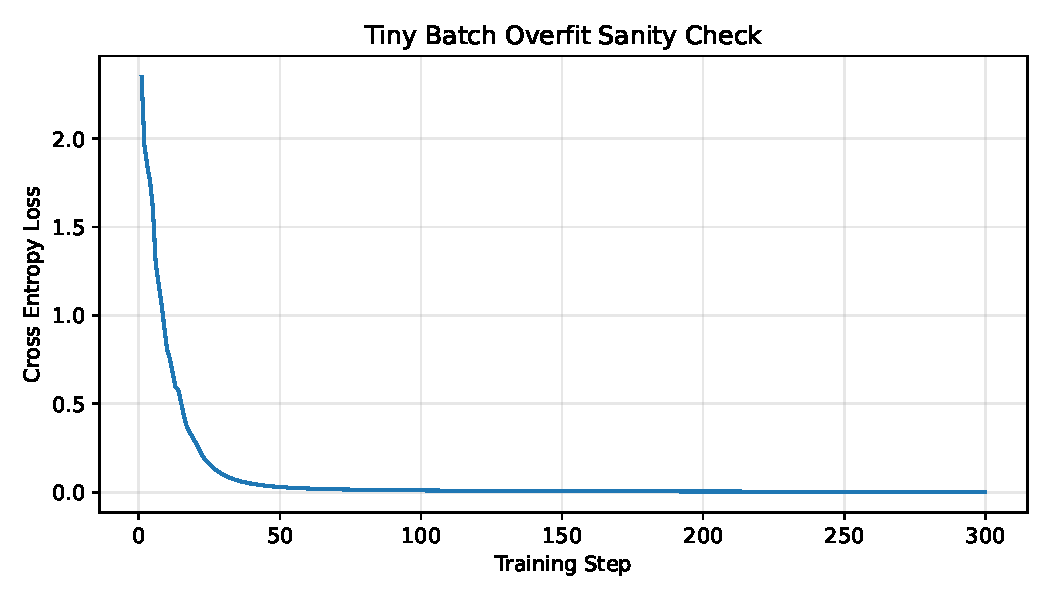
\includegraphics[width=0.6\linewidth]{overfit.pdf}
\caption{Tiny-batch overfit check (\texttt{python main.py sanity}): on 32
fixed images, the training loss falls from 2.35 to 0.002 in 300 steps,
showing that the full forward and backward pipeline can fit data.}
\label{fig:overfit}
\end{figure}
\begin{figure}[t]
\centering
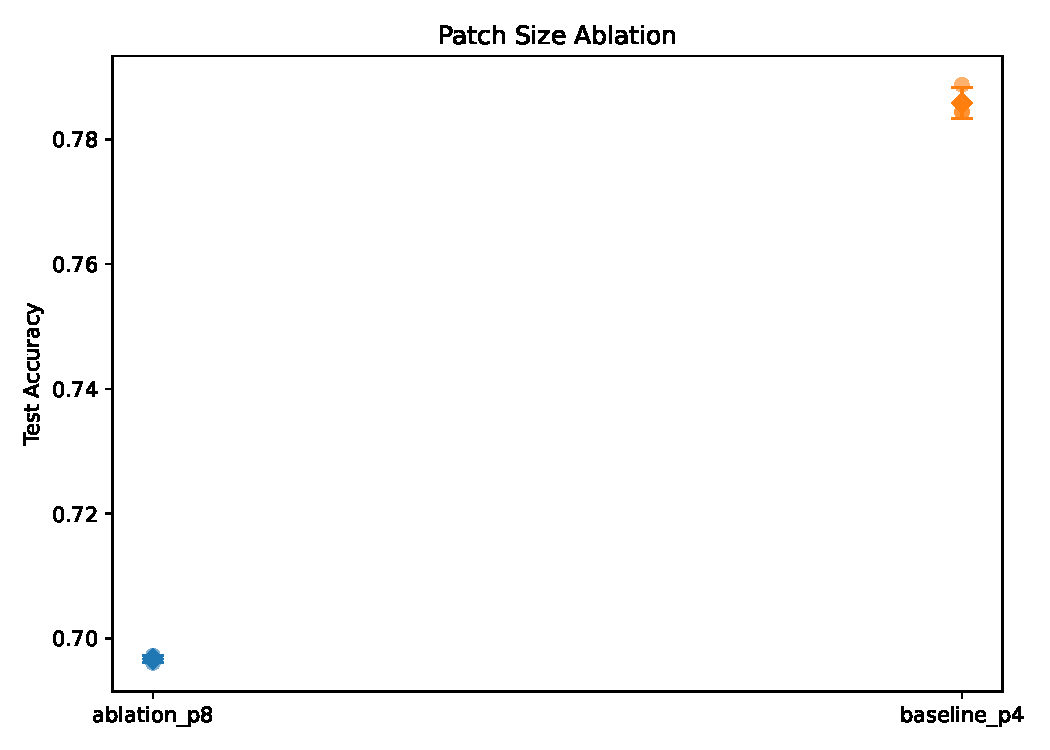
\includegraphics[width=0.6\linewidth]{ablation_acc.pdf}
\caption{Test accuracy for patch size 4 and 8 over three seeds.}
\label{fig:ablation}
\end{figure}
\end{document}